% Author: Izaak Neutelings (July 2018)
% page 8 https://archive.org/details/StaticAndDynamicElectricity
% https://tex.stackexchange.com/questions/56353/extract-x-y-coordinate-of-an-arbitrary-point-on-curve-in-tikz
% https://tex.stackexchange.com/questions/412899/tikz-calculate-and-store-the-euclidian-distance-between-two-coordinates

\documentclass[border=3pt,tikz]{standalone}
\usepackage{amsmath} % for \dfrac
\usepackage{bm}
\usepackage{physics}
\usepackage{tikz,pgfplots}
\usetikzlibrary{angles,quotes} % for pic (angle labels)
\usetikzlibrary{calc}
\usetikzlibrary{decorations.markings}
\tikzset{>=latex} % for LaTeX arrow head

\usepackage{xcolor}
\tikzstyle{charged}=[top color=blue!20,bottom color=blue!40,shading angle=10]
\tikzstyle{charge+}=[very thin,top color=red!60,bottom color=red!80!black!55,shading angle=-5]
\tikzstyle{charge-}=[very thin,top color=blue!40,bottom color=blue!80!black!55,shading angle=10]
\tikzstyle{measure}=[fill=white,midway,inner sep=2]
\def\tick#1#2{\draw[thick] (#1) ++ (#2:0.15) --++ (#2-180:0.3)}


\begin{document}



% ROD ELECTRIC FIELD
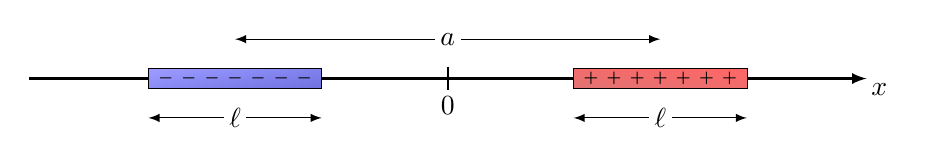
\begin{tikzpicture}
  \def\L{2.2}  % rod length
  \def\t{0.25} % rod thickness
  \def\a{5.4}  % distance between rod centers
  \def\h{0.5}  % height measures
  \def\N{7}    % number of charge signs per rod
  \def\xmax{{0.7*(\L+\a)}}
  
  % AXIS
  %\draw[dashed,very thin] (0,0) -- (0,-2.5*\h) (0,0) -- (0,2.5*\h);
  %\draw[dashed,very thin] (-\a/2,0) --++ (0,1.6*\h);
  %\draw[dashed,very thin] ( \a/2,0) --++ (0,1.6*\h);
  \draw[->,thick] (-\xmax,0) -- (\xmax,0) node[below right=-2] {$x$};
  \tick{0,0}{90} node[fill=white,inner sep=2,below] {$0$};
    
  % MEASURES
  \draw[<->] (-\a/2,\h) --++ (\a,0) node[measure] {$a$};
  \draw[<->] (-\L/2-\a/2,-\h) --++ (\L,0) node[measure] {$\ell$};
  \draw[<->] (-\L/2+\a/2,-\h) --++ (\L,0) node[measure] {$\ell$};
  
  % ROD
  \draw[charge-] (-\L/2-\a/2,-\t/2) rectangle ++(\L,\t);
  \draw[charge+] (-\L/2+\a/2,-\t/2) rectangle ++(\L,\t);
  \foreach \i [evaluate={\x=(\i-0.25)*\L/(\N+0.5);}] in {1,...,\N}{
    \node[scale=0.6] at (-\L/2-\a/2+\x,0) {$\bm-$};
    \node[scale=0.6] at (-\L/2+\a/2+\x,0) {$\bm+$};
  }
  
\end{tikzpicture}



\end{document}
